\documentclass{article}


\usepackage[papersize={8.27in,11.69in},hmargin=0.5in,tmargin=1.055in,bmargin=1.055in,includehead]{geometry}
% paper size if 6in x 9in which is standard international size
% margin from top is 0.7in including header
% margin from bottom is 0.6in including footer
% book of two sided pages is specified, with horizontal margin of 0.6in
% binding offset is an additional 0.1in from centre fold.
% REAL textwidth is therefore 6 - 2*0.6 -0.1 = 4.7in = 11.938cm, 0.45\textwidth = 5.3721 cm with 3 margins of 0.3979cm
\usepackage{multicol}
\setlength{\columnsep}{0.27in}
%
\usepackage[
    backend=bibtex,
    %backend=biber, 
    natbib=true,
    style=numeric,
    sorting=none,
    backref=true
]{biblatex} %,style=verbose-trad2
%\addbibresource{bib.bib}
\bibliography{bib}


\usepackage[explicit]{titlesec}
\usepackage{titletoc}
\usepackage{lmodern}
\usepackage{epigraph}
\usepackage{xpatch}  % All above used in titling
%
\usepackage{tikz}
%
\usepackage{pgfplots} % for better precision plots
\pgfplotsset{compat=1.10} % for newer version?
\usepgfplotslibrary{fillbetween} % for shading pgfplots

\usepackage{graphicx}
\usepackage{wrapfig} % for odd wrapping of text around figure
%
\usepackage{textcomp} % for currency %\usepackage[gen]{eurosym}
%
\usepackage{lipsum} %for filler text only
%
%\usepackage{bold-extra} % Used in Game Theory Section for bold sc's
\usepackage[T1]{fontenc}
%
\usepackage{mathtools}
\usepackage{amsthm}
\usepackage{bm} %for bold greeks
\usepackage{booktabs} %for better standard tables
\usepackage{longtable} %used for acronymns table
\usepackage{array} % for customising paragraph p columns alignment
\usepackage{tablefootnote} % obvious
\usepackage{arydshln} %for dotted v lines in tables
%
\usepackage{glossaries}
\usepackage{caption}
\usepackage{subcaption}
%
\usepackage{enumerate} %for lists
%
\usepackage{fancyhdr} %for custom page headers
%
\usepackage{imakeidx} % for indexing

%%% TIKZ Predefinitions
\usetikzlibrary{patterns}
\usetikzlibrary{decorations}
\tikzstyle{block} = 
    [rectangle, draw
     % , fill=blue!20
      , text width=7.5em
      , text centered
      , node distance=3.5cm
      , rounded corners
      , minimum height=2em
      , scale =0.8]
\tikzstyle{blockL} = 
    [rectangle, draw
     % , fill=blue!20
      , text width=7.5em
      , align=left
      , node distance=3.5cm
      , rounded corners
      , minimum height=2em
      , scale =0.8]
\tikzstyle{block20} = 
    [rectangle, draw
     % , fill=blue!20
      , text width=9em
      , text centered
      , node distance=3.5cm
      , rounded corners
      , minimum height=2em
      , scale =0.8]
      \tikzstyle{block40} = 
    [rectangle, draw
     % , fill=blue!20
      , text width=10.5em
      , text centered
      , node distance=3.5cm
      , rounded corners
      , minimum height=2em
      , scale =0.8]
 \tikzstyle{Vblock} = 
    [rectangle, draw=none
     % , fill=blue!20
      , text width=15em
      , text centered
      , node distance=3.5cm
      , rounded corners
      , minimum height=2em
      , scale =0.8]
\tikzstyle{Lblock} = 
    [rectangle, draw
     % , fill=blue!20
      , text width=35em
      , text centered
      , node distance=3.5cm
      , rounded corners
      , minimum height=2em
      , scale =0.8]
\tikzstyle{virtual} = [coordinate]
%%%%%%%%%%%%%%%%%%%%


\usepackage{lipsum}
\AtBeginDocument{\renewcommand{\bibname}{\centerline References}}
\begin{document}

{
	\centering
	\vspace{1cm}
	{\scshape\Huge\ [TITLE TBD] \par}
	\vspace{1cm}
	{\scshape\Large --- \par}
	\vspace{0.9cm}
	\begin{center}{Mohammed Al-Jaff, Albin Stjerna, Pontus Hallden, J Hamish M Darbyshire}\\
	Uppsala University, Uppsala, Sweden
	\end{center}
}

\begin{multicols}{2}

\section*{Abstract}

\textbf{ \textit { We do something with some data }}

\section*{Background}

\section*{Methods}
\subsection*{Data Formats}
In December 2017 it was publicly announced by 4iQ, a US digital security company, \cite{data2017breach} that a large database of plaintext username password pairs was downloadable from the world wide web. The validity of the dataset is noted by its prominent status amongst hacking communities and the anecdotal evidence that one of the author's username password pairs was correctly identified in addition to one of our colleagues! However, we also suspect many passwords to be outdated, and some must be considered fake as the result of failed phishing attacks. We make no attempt to verify the integrity of all of the data and do not believe a lack of full integrity to have any meaningful impact on our results.
\par Our raw dataset, then, is a series of plaintext files, organised within a hierarchical directory, sorted alphabetically by the initial characters of any given file. There are approximately 700 files of variable file size. Each line of every file is a specific datapoint and comprises a username-password pair with a colon separator. For example, 'joe@someaccount.com:joespassword1' is a line entry in a file that would be assigned to the directory structure '/j/o/'. Collectively there are approximately 1.4 billion lines to process.
\par [\_\_INPUT\_\_ on what drive do we store the data and why choose that?]

\subsection*{Operations}
We employ Apache Spark~\cite{apache-spark} to coordinate our operations across multiple distributed nodes. Each node is created to the following specifications; [\_\_INPUT\_\_ nodes have spec?]
\par We outline the operations performed by the distributed node cluster below.
\begin{enumerate}[1.]
\item We perform a generic map-reduce operation designed to discard usernames from the raw dataset and return a list of unique passwords with an associated count for each. We save this data to our filesystem for further processing.
\item We analyse, with regular expressions, each unique password detected in 1 to further detect alpha strings, digit strings and special strings, in accordance with the definition outlined by Weir et al. \cite{weir2009password}. We record a count associated with each unique string detected. We also process the overall structure of the password delineated into the subcategories. The results serve as the final objective and we draw contextual conclusions as a point of interest.
\end{enumerate}

\subsection*{Computational Experiments}
We perform both strong and weak type experiments on the two different operation types, to evaluate the collective performance of the distributed nodes.

\begin{enumerate}[1.]
\item We evaluate the total time to completion of operation 1 with variable numbers of identical worker processing nodes.
\item We evaluate the time to completion of operation 1 applied to a subset of data, with variable numbers of workers, and the size of the subset linearly proportional to the number of workers.
\item We evaluate the total time to completion of operation 2 with variable numbers of identical workers.
\item We evaluate the time to completion of operation 2 applied to a subset of data, with variable numbers of workers, and the size of the subset linearly proportional to the number of workers.
\end{enumerate}

\subsubsection*{Data Storage and Transfer}

\begin{figure}[H]
  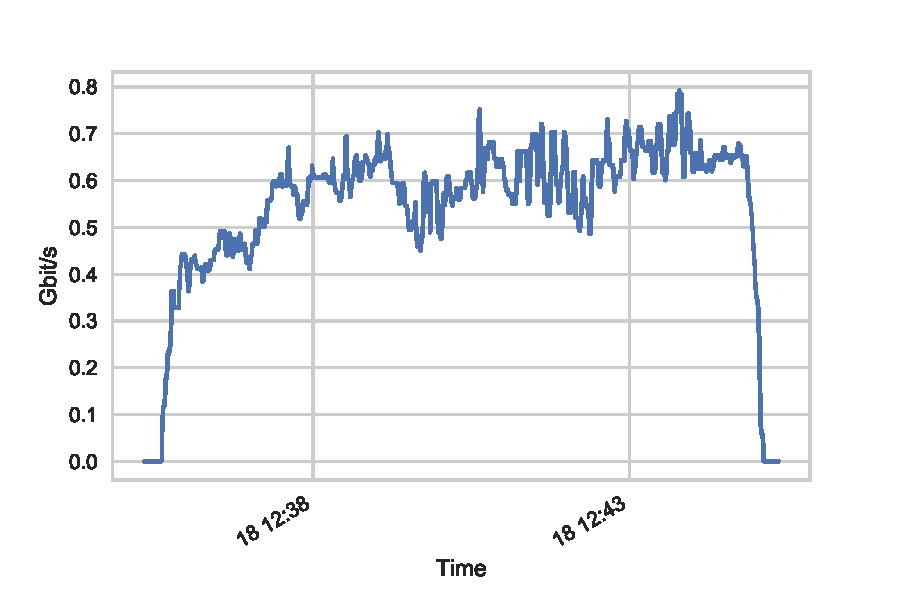
\includegraphics[width=\linewidth]{rolling}
  \caption{Outgoing network traffic on the NFS file server during a
    brief full-cluster experiment run showing likely network
    saturation. The figure shows a moving median to reduce the noise in
    the measurements.}\label{fig:rolling-data}
\end{figure}


A preliminary experiment where the data was distributed across the full
$11$-node cluster using Network File System (NFS) running on a separate
node was performed. During the execution of a simple counting task
across the full dataset, measurements of network traffic at the file
server was taken using \textit{bwm-ng}. A rolling median graph of the
outgoing network traffic, showing what is most likely network bandwidth
saturation, can be seen in Figure~\ref{fig:rolling-data}.

\section*{ Results}

\section*{ Discussion}
\cite{kelley2012guess} \cite{weir2009password}

\section*{ Conclusion}

{\color{red}

We plan to source and store a large number of username-password files. We will batch process this data using distributed computing to map reduce the file into password-count pairs. We will develop a malleable high level interface to extract information from the map reduced file, saving results to disk in a manageable way.  We will use Apache Spark and discuss its effectiveness.

\section*{Dataset}
We source a data set consisting of 1.4 billion clear text password and username pairs, totalling to about 50GB of data. The dataset was originally found as an unprotected single file on the dark web by employees of the internet security company 4IQ. According to 41Q, the contents of the dataset were aggregated from many previous leaked credential breaches in the past. The dataset is available through a magnet link from https://github.com/philipperemy/tensorflow-1.4-billion-password-analysis

\section*{Steps}

\begin{enumerate}[(i)]

\item Source the data and make it available on the cluster. Make references in the report to an optimal form of storage for thses text files.
\item Process the files with map reduce to return password-count pairs and save this information for future use.
\item Develop an interface to return custom statistics from the map reduced files, and be capable of storing the results. Considering statistics such as, how many passwords contain numbers? How many passwords contain symbols? How many passwords don't contain the letter 'e'? The most common bi-grams? etc..
\item Monitor the cluster and perform tests to evaluate its performance. Such as the effect of scaleability in the horizontal direction.
\item Discuss expectations and challenges if the dataset was much larger.

\end{enumerate}
}



%Some citation example \cite{examplebib}
\printbibliography

\end{multicols}
\end{document}
